\documentclass[11pt]{article}
\usepackage[margin=0.8in]{geometry}
\usepackage{amsmath,amssymb,amsthm,booktabs,graphicx,longtable,tikz,pgfplots}
\usepackage[colorlinks=true,urlcolor=blue,linkcolor=blue]{hyperref}
\pgfplotsset{compat=1.18}
\newtheorem{theorem}{Theorem}
\newcommand{\F}{\mathbf F}
\setlength{\emergencystretch}{2em}
\title{Measuring cubic norm-one class admission\\over 192--252-bit fields}
\author{ISO-1 research evidence}
\date{9 October 2026}
\begin{document}
\maketitle
\newcommand{\TotalCurves}{512}
\newcommand{\TotalOrdinary}{512}
\newcommand{\TotalAdmitted}{323}
\newcommand{\TotalWitnesses}{0}
\newcommand{\TotalUnresolved}{323}
\newcommand{\TotalVertices}{32484}
\newcommand{\TotalEdgesTwo}{54216}
\newcommand{\TotalEdgesThree}{38093}
\newcommand{\ComponentExhausted}{219}
\newcommand{\VertexCapped}{104}
\newcommand{\SearchTimeCapped}{0}
\newcommand{\FailedCells}{0}
\newcommand{\PrecisionInterval}{{$[0,1]$}}

\begin{abstract}
We independently sample \TotalCurves{} full-2-torsion curve models in ten
finite fields of bit lengths 192--252 and extension degrees 6, 10, and 14.
The necessary conductor condition admits \TotalAdmitted{} of the
\TotalOrdinary{} ordinary curves. Every admitted curve has a verified
full-4-torsion representative at distance at most one rational 2-isogeny,
after choosing the trace sign. We prove that this torsion property is exactly
what the admission condition characterizes. The bounded degree-2/3 searches
find \TotalWitnesses{} norm-one weak witnesses among these independent starts;
\TotalUnresolved{} admitted class labels remain unresolved. All ten separately
constructed positive controls recover their known weak class. A norm-fiber
count also bounds the probability that a uniform source model is already
weak by $3/(p^2-1)$, separating direct model density from class reach.
The class labels concern the cubic norm-one branch. A separate exact
quartic control demonstrates that the quadratic branch in Joux--Vitse
can occupy a class empty in the cubic census.
\end{abstract}

\section{The measured population}
Put $q=p^2$, $K=\F_{q^n}$, $Q=q^n$, and
$N=(Q-1)/(q-1)$, with odd $n\ge3$. The weak family is
$y^2=x(x-\alpha)(x-\alpha^q)$, up to $K$-isomorphism.
An ordinary weak class must satisfy
\[
 t\equiv\pm(Q+1)\pmod {16},\qquad 4\mid f_\pi,
\]
where $f_\pi$ is the conductor of the Frobenius order, separately from
the endomorphism-order conductor. The previous theorem proves this
condition in every such odd extension. The new measurement samples
$(u,v)$ uniformly among distinct nonzero elements of $K$ and counts
$E:y^2=x(x-u)(x-v)$. Consequently the population is uniform in these
ordered root pairs and includes both quadratic twist signs; it is not
uniform in traces or in isogeny classes. Equal traces remain separate rows.

\begin{center}
\begin{tabular}{rrrrrl}
\toprule
Bits & Degree & $p$ & Samples & Admitted & Rate (Wilson 95\%)\\
\midrule
192 & 6 & 4294967291 & 64 & 39 & 60.9\% (48.7--71.9)\\
204 & 6 & 17179869143 & 64 & 41 & 64.1\% (51.8--74.7)\\
216 & 6 & 68719476731 & 64 & 43 & 67.2\% (55.0--77.4)\\
228 & 6 & 274877906899 & 64 & 40 & 62.5\% (50.3--73.3)\\
240 & 6 & 1099511627689 & 64 & 42 & 65.6\% (53.4--76.1)\\
252 & 6 & 4398046511093 & 64 & 42 & 65.6\% (53.4--76.1)\\
192 & 10 & 602233 & 32 & 18 & 56.2\% (39.3--71.8)\\
252 & 10 & 38543917 & 32 & 23 & 71.9\% (54.6--84.4)\\
192 & 14 & 13421 & 32 & 18 & 56.2\% (39.3--71.8)\\
252 & 14 & 262139 & 32 & 17 & 53.1\% (36.4--69.1)\\
\bottomrule
\end{tabular}

\end{center}
Intervals are Wilson 95\% intervals for independently sampled curve
admission. Bit length means $\lfloor\log_2 Q\rfloor+1$; all fields meet
the requested integer bit sizes. Six degree-6 primes are the largest primes
below $2^{32},2^{34},\ldots,2^{42}$. The degree-10 and degree-14 endpoint
primes are the largest below the corresponding integer root of $2^b-1$.
Exact cardinalities, irreducible moduli, coefficients, full ICV1 identities,
and raw hashes are in \href{population_run1/curve_records.json}{the records}.

\begin{center}
\begin{tikzpicture}
\begin{axis}[width=0.96\linewidth,height=6.7cm,ymin=0,ymax=1,
 xlabel={Field cell: integer bits / total extension degree},
 ylabel={Ordinary-curve admission fraction},
 xtick={1,2,3,4,5,6,7,8,9,10},
 xticklabels={192/6,204/6,216/6,228/6,240/6,252/6,192/10,252/10,192/14,252/14},
 x tick label style={rotate=40,anchor=east,font=\small},
 ytick={0,0.25,0.5,0.625,0.75,1},yticklabels={0,0.25,0.5,0.625,0.75,1},grid=major,
 legend style={at={(0.5,1.02)},anchor=south,draw=none,font=\small},
 error bars/y dir=both,error bars/y explicit]
 \addplot+[only marks,mark=*,color=blue,error bars/y dir=both,error bars/y explicit]
 table[x=field,y=admission_rate,y error minus=error_low,y error plus=error_high,col sep=comma]{plot_data.csv};
 \addlegendentry{Measured admission, Wilson 95\%}
 \addplot[gray,dashed,domain=0.5:10.5] {0.625};
 \addlegendentry{Uniform mod-16 matrix model: $5/8$}
\end{axis}
\end{tikzpicture}
\end{center}
The dashed reference is an exact count under a specified matrix model:
among the 512 matrices modulo 16 congruent to the identity modulo 2
with determinant $Q\bmod16\in\{1,9\}$, exactly 320 have the admitted
trace. It is not a proved finite-field population law. Each field is its
own sampling stratum; the pooled admission is a summary of this fixed design.

\section{What the conductor condition characterizes exactly}
\begin{theorem}[A full-4-torsion representative within one edge]
Let $K$ have odd cardinality $Q\equiv1\pmod4$, and let $E/K$ have full
rational 2-torsion. Then $16\mid\#E(K)$ if and only if $E$ itself, or
one of its rational degree-2 quotients, has full rational 4-torsion.
Thus $t\equiv\pm(Q+1)\pmod {16}$ is equivalent to this property for
one of the two quadratic twist signs.
\end{theorem}
\begin{proof}
A full-4-torsion representative has group order divisible by 16,
and an isogeny preserves the order. Conversely, the 2-primary group
of an elliptic curve has at most two cyclic factors. If $E[4](K)$
is not full and $16\mid\#E(K)$, full rational 2-torsion forces a
rational point $P$ of order 8. Put $T=2P$ and $A=2T=4P$.
Translate $A$ to $(0,0)$ and write
\[
 E:y^2=x(x-u)(x-v)=x(x^2+ax+b),\qquad a=-(u+v),\quad b=uv.
\]
The duplication formula is
\[
 x(2R)=\frac{(x(R)^2-b)^2}{4y(R)^2}.
\]
Since $2T=A$, write $x(T)=s$ with $s^2=b$. Applying the translated
duplication formula at each rational root shows that $x(2P)-e_i$
is a square for all three roots $e_i$. In particular, $s=x(T)$ is
a nonzero square. Since $T$ lies on $E$, also
$a+2s=y(T)^2/s^2$ is a nonzero square.

The degree-2 quotient by $A$ has equation
\[
 E':y^2=x[x^2-2ax+(a^2-4b)]
\]
and roots $0,a+2s,a-2s$. The product of the two nonzero roots is
$(u-v)^2$, so both roots are squares. Their difference is $4s$,
also a square. Because $-1$ is a square in $K$, every signed root
difference is a square. The standard rational halving formulas give
independent halves of two distinct 2-torsion points, so $E'[4]$ is full.
For the trace pair, one order is divisible by 16 exactly under the
displayed congruence, and both twists retain full rational 2-torsion.
\end{proof}
The cleared duplication identity has record
\texttt{IDC1h40099ec00a503c89}; the earlier rational-halving and
degree-2-map identities retain their existing certificates.
An independent exhaustive check covers all 5,264 ordered root pairs in
eight fields of cardinalities 5 through 49. It independently factors each
quotient's 2-torsion polynomial and point-counts each quotient. All 1,336
order-divisible-by-16 cases agree with the one-edge equivalence; 592
already have full 4-torsion and 744 require an edge. The exact output is
retained in \texttt{torsion\_exact.txt}.
Every admitted large-field sample passes explicit halving and map checks. This theorem
explains the exact torsion feature observed at large field sizes. It leaves
the additional norm-one class-intersection condition as a distinct question.

\section{Direct weak-model density}
\begin{theorem}[Norm-fiber bound]
For the sampled full-2-torsion model, put $\lambda=v/u$.
Then $\lambda$ is uniform in $K\setminus\{0,1\}$, and
\[
 \Pr(E\text{ already has a weak model})
 \le\frac{3(N-1)}{Q-2}<\frac{3}{q-1}.
\]
\end{theorem}
\begin{proof}
Writing $\mathcal N=N_{K/\F_q}$, the three choices of translated root
give the exact direct-model conditions
\[
 \mathcal N(\lambda)=1,\qquad
 \mathcal N(\lambda-1)=-1,\qquad
 \mathcal N((\lambda-1)/\lambda)=1.
\]
For example, equality of the norms of $u$ and $v$ is the first condition.
Hilbert 90 gives the required conjugate pair; multiplying its parameter
by an element of $\F_q^\times$ selects the square class needed for a
$K$-isomorphism, since the extension degree is odd. The other two
choices give the remaining conditions. Each event has $N-1$ parameters:
the norm map has fibers of size $N$, and the corresponding linear or
fractional-linear substitution removes exactly one excluded parameter
from that fiber. The union bound proves the first inequality.
Since $(q-1)N=Q-1$, its numerator gives
$3(N-1)/(Q-2)=3(Q-q)/[(q-1)(Q-2)]<3/(q-1)$.
\end{proof}
The geometric-sum identities at odd degrees 3, 5, and 7 have records
\texttt{IDC1hc1132e34bb8c94e8}, \texttt{IDC1h547a8ae22b837173}, and
\texttt{IDC1hcacc5ce8020b68ac}. Each certificate passes 32 recorded plus
64 additional evaluations; exact GP symbolic expansion returns zero.
Exhaustive direct-locus checks cover 15,623, 117,647, and 59,047
parameters at $(p,n)=(5,3),(7,3),(3,5)$, respectively. Each of the
three event counts is exactly $N-1$.

\begin{center}
\begin{tabular}{rrrl}
\toprule
Bits & Degree & $p$ & Direct-model probability upper bound\\
\midrule
192 & 6 & 4294967291 & $1.626\times10^{-19}$\\
204 & 6 & 17179869143 & $1.016\times10^{-20}$\\
216 & 6 & 68719476731 & $6.353\times10^{-22}$\\
228 & 6 & 274877906899 & $3.970\times10^{-23}$\\
240 & 6 & 1099511627689 & $2.482\times10^{-24}$\\
252 & 6 & 4398046511093 & $1.551\times10^{-25}$\\
192 & 10 & 602233 & $8.272\times10^{-12}$\\
252 & 10 & 38543917 & $2.019\times10^{-15}$\\
192 & 14 & 13421 & $1.666\times10^{-8}$\\
252 & 14 & 262139 & $4.366\times10^{-11}$\\
\bottomrule
\end{tabular}

\end{center}
This is a bound on the randomly drawn source model, separately from the
presence of a weak representative anywhere in its isogeny class. Increasing
the odd relative degree while fixing the total bit size makes the base
field smaller and increases this direct-model density bound.

\section{Witness searches and the remaining class labels}
All witness and exclusion labels here select the displayed cubic norm-one
family. The broader quadratic branch is tested separately below.
For relative degrees 5 and 7, the rows verify generalized norm-one arithmetic
and torsion; the cited genus-3 cover applies to relative degree 3.
For each admitted ordinary sample, the search follows rational isogenies
of degrees 2 and 3, retaining vertices with full rational 2-torsion.
The fixed limits are 256 distinct $j$-invariants, 90 seconds for the search,
and 240 seconds for the complete GP child. Each retained edge checks its
2-torsion roots and three mapped points. A witness must satisfy the exact
norm equalities and pass a fresh point count with the selected source trace.
The two trace signs share weak-class presence because the family is closed
under quadratic twisting.

The population run tests \TotalVertices{} vertices and evaluates
\TotalEdgesTwo{} retained degree-2 and \TotalEdgesThree{} degree-3 edges.
It finds \TotalWitnesses{} witnesses. The \TotalUnresolved{} admitted
classes remain unresolved: \ComponentExhausted{} searches exhaust their
restricted component and \VertexCapped{} reach the vertex cap.
There are \SearchTimeCapped{} search-time caps and \FailedCells{} failed
or parent-capped cells. Exhausting this restricted graph does not enumerate
the whole isogeny class. With no exact labels for these admitted large-field
classes, the identified precision interval is \PrecisionInterval{}.
The previously observed small-prime census precision therefore remains a
measurement of its own population.

\begin{center}
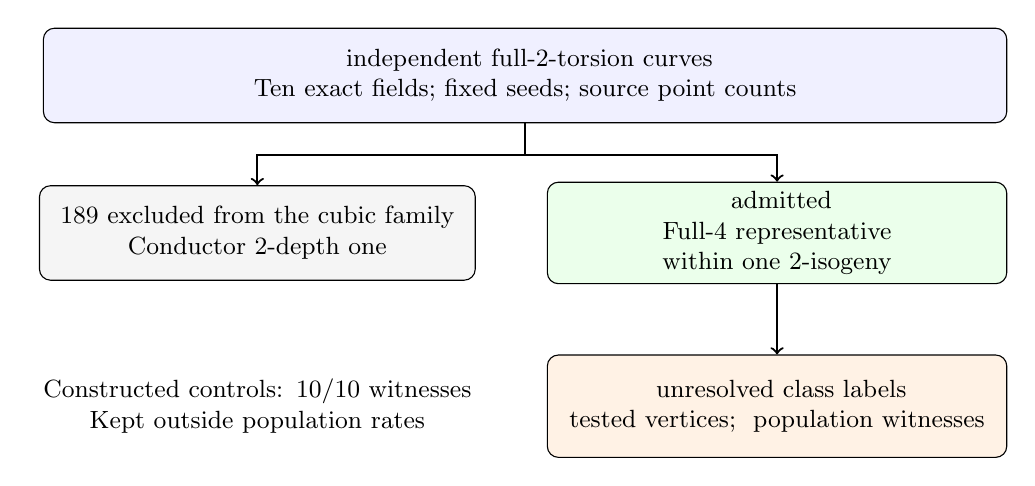
\begin{tikzpicture}[every node/.style={align=center,font=\small}]
\node[draw,rounded corners,fill=blue!6,text width=12cm,minimum height=1.2cm] (all)
 {\TotalCurves{} independent full-2-torsion curves\\Ten exact fields; fixed seeds; source point counts};
\node[draw,rounded corners,fill=gray!8,text width=5.3cm,minimum height=1.2cm] (excluded) at (-3.4,-2)
 {189 excluded from the cubic family\\Conductor 2-depth one};
\node[draw,rounded corners,fill=green!8,text width=5.6cm,minimum height=1.2cm] (admitted) at (3.2,-2)
 {\TotalAdmitted{} admitted\\Full-4 representative within one 2-isogeny};
\node[draw,rounded corners,fill=orange!10,text width=5.6cm,minimum height=1.3cm] (unresolved) at (3.2,-4.2)
 {\TotalUnresolved{} unresolved class labels\\\TotalVertices{} tested vertices; \TotalWitnesses{} population witnesses};
\node[text width=5.6cm] at (-3.4,-4.2)
 {Constructed controls: 10/10 witnesses\\Kept outside population rates};
\draw[->,thick] (all.south) -- ++(0,-0.4) -| (excluded.north);
\draw[->,thick] (all.south) -- ++(0,-0.4) -| (admitted.north);
\draw[->,thick] (admitted.south) -- (unresolved.north);
\end{tikzpicture}
\end{center}

All ten constructed controls start off the direct weak locus, at a
2-isogeny neighbor of a norm-one curve. The search finds a weak endpoint
after testing two vertices in each case. Both source and endpoint are
point-counted independently. These controls demonstrate witness detection
at the requested sizes and are excluded from population proportions.
The source and endpoint of one 252-bit control, including full ICV1
identities and the kernel, are shown in
\href{verified_control.svg}{the evidence-linked diagram}.

The small-field validation has 64 independent $\F_{7^6}$ source models.
The complete exact census labels 42 of their classes weak and 22 zero.
Of 49 admitted starts, the search finds 38 witnesses. Among 11 restricted
component closures, seven are exact zeros and four are weak classes that
this restricted search misses. All 15 rejected classes are exact zeros.
This supplies an explicit validation of the unresolved-label policy.
Four additional constructed small-field controls also succeed.

\section{Reproducibility and requirement status}
The pre-run \href{PROTOCOL.md}{protocol} fixes the sample law, seeds,
fields, caps, and label rules. A compiled Rust driver runs four PARI/GP
2.17.3 workers. The host is an Apple M4 Pro, 14 logical CPUs, 48 GiB
memory, macOS Darwin 25.6.0 arm64. The source hash, native executable hash,
GP executable hash, command parameters, exit status, wall resource receipt,
and both raw output hashes are retained for every attempted cell. Resource
times are from a shared host and do not constitute controlled timing ratios.
The native checker rebuilds summary tables and canonical model identities
from the raw records and rejects changed receipts or labels. An additional
GP replay reconstructs every model from the recorded modulus and roots,
checks its short coefficients and $j$, and verifies all saved witness routes.

\begin{center}
\begin{tabular}{p{0.42\linewidth}p{0.50\linewidth}}
\toprule
Requested requirement & Current evidence status\\
\midrule
192--252-bit fields and larger degrees & Verified: 512 counted samples in ten fields, degrees 6, 10, 14.\\
Necessary condition and torsion measurement & Verified: \TotalAdmitted{} admissions and matching full-4 representatives.\\
Explicit weak-model search & Verified bounded result: population \TotalWitnesses{}, constructed controls 10/10.\\
Large-field weak-class prediction precision & Partial: \TotalUnresolved{} admitted labels unresolved; exact CM support construction remains the missing scalable step.\\
Theorem and reproducible report & Proofs, four algebra records, native checks, raw receipts, editable visuals, and this PDF.\\
\bottomrule
\end{tabular}
\end{center}
The existing cubic-family CM norm-one criterion gives a necessary-and-sufficient
class decision by intersecting the norm-one locus with selected CM orders.
Its order-support construction is separate from the constant-degree norm
checks. A recorded preflight on the first admitted 192-bit source obtains
$f_\pi=8$ and a 188-bit fundamental discriminant, then \texttt{polclass}
stops with \texttt{overflow in t\_INT-->long assignment}. This is an
observed implementation limit in the exact support path; its raw output,
error, and fail-closed receipt are retained in \texttt{cm\_preflight.*}.
The next algorithmic step is an on-demand CM intersection or a
certified class-action traversal at these bit sizes, followed by exact
positive and zero labels for independently sampled admitted classes.
The earlier complete small-prime census continues under its finite local
worker; it is not pooled into this experiment.

\paragraph{Primary implementation reference.}
PARI's \href{https://pari.math.u-bordeaux.fr/dochtml/html/Elliptic_curves.html}{elliptic-curve documentation}
specifies finite-field \texttt{ellcard}, polynomial-kernel \texttt{ellisogeny},
and \texttt{ellisogenyapply}. The program retains each witness kernel and
the actual target model produced by the polynomial map, so the route can
be replayed without choosing another isomorphic model.
\section{Contribution relative to Joux--Vitse}
The cover-and-decomposition method is credited to
\href{https://www.iacr.org/archive/eurocrypt2012/72370010/72370010.pdf}{Joux--Vitse}.
Their Section 4.1 includes both linear and quadratic $h\in\F_q[x]$ in
$y^2=h(x)(x-\alpha)(x-\alpha^q)$ and discusses class reach heuristically.
Our cubic norm-one theorem and census concern the linear branch.

We tested 100 nonsplit quadratic models over $\F_{7^6}$ with fixed
$d\in\F_{49}$ nonsquare. Forty-six ordinary traces fail the cubic
conductor predicate. Complete affine-$x$ enumeration, with two infinity
points, independently verifies three selected models:
\begin{center}
\begin{tabular}{rrrr}
\toprule
Trace & Exact cardinality & $f_\pi$ & $v_2(f_\pi)$\\
\midrule
$-38$ & 117,688 & 18 & 1\\
$-10$ & 117,660 & 26 & 1\\
610 & 117,040 & 72 & 3\\
\bottomrule
\end{tabular}
\end{center}
Thus the exact cubic zero at trace $\pm610$ has a published-family
quadratic representative. It is not an empty class for the full family.
The equations, parameters, exact counts, and full model identities
are retained in \href{quadratic_curve_records.json}{the three quadratic records}.

The standard branch-point coordinate change sets
$c_3=f'(\alpha)$, $c_2=f''(\alpha)/2$, $c_1=f'''(\alpha)/6$ and
\[
 X=\frac{c_3}{x-\alpha},\quad
 Y=\frac{c_3y}{(x-\alpha)^2},\quad
 Y^2=X^3+c_2X^2+c_3c_1X+c_3^2.
\]
Each control checks the inverse and three mapped points.
The cleared coordinate identity has record
\texttt{IDC1hb01002991ea88fb4}.
Seventy-five retained cubic positive models also have constructive
Hilbert--90 parameters and explicit coordinate changes verified during
the independent replay.

The contribution to develop is the subfamily's conductor restriction,
exact class evidence, and orbit census formulas. The one-edge torsion
explanation uses standard arithmetic: the root-difference halving
criterion is already in
\href{https://pure.rug.nl/ws/portalfiles/portal/14410242/2002JNumberThAuer.pdf}{Auer--Top},
Lemma 2.1 and Proposition 2.1. Priority for the norm-one application
against the wider cover literature remains to be checked.
The next stronger result is a complete two-branch criterion with an
explicit construction and a verified cost on independently sampled classes.
\href{PRIOR_WORK.md}{The attribution and scope comparison} gives the
evidence and remaining novelty checks.
\end{document}
